\documentclass[11pt,a4paper]{article}
\usepackage[margin=22mm]{geometry}
\usepackage{fontspec}
\setmainfont{Times New Roman}
\usepackage{graphicx}
\usepackage{longtable}
\usepackage{array}
\usepackage{booktabs}
\usepackage{xcolor}
\usepackage{hyperref}
\hypersetup{colorlinks=true,urlcolor=blue!45!black,linkcolor=black}
\usepackage{fancyhdr}
\pagestyle{fancy}
\fancyhf{}
\fancyhead[L]{\small Temporal event graphs for hypoglycemia prediction}
\fancyhead[R]{\small Working draft}
\fancyfoot[C]{\thepage}
\setlength{\headheight}{14pt}
\setlength{\parindent}{0pt}
\setlength{\parskip}{6pt}
\setlength{\emergencystretch}{3em}
\renewcommand{\arraystretch}{1.2}
\begin{document}
{\raggedright\hyphenpenalty=10000\LARGE\bfseries Temporal Event Graphs for Short-Horizon Hypoglycemia Prediction in Type 1 Diabetes: A Controlled Retrospective Development Study\par}
\vspace{8pt}
Authors: [AUTHOR NAMES AND ORDER TO BE CONFIRMED]

Affiliations: [INSTITUTIONS AND DEPARTMENTS TO BE CONFIRMED]

Corresponding author: [NAME AND EMAIL TO BE CONFIRMED]

Working manuscript | Evidence snapshot: 20 October 2026 | Standard journal format

\section*{Abstract}
\textbf{Background:} Linking recorded insulin and carbohydrate events to continuous glucose monitoring (CGM) histories may improve hypoglycemia prediction, but requires comparison with an equally informed sequence model.

\textbf{Objective:} To compare temporal event graphs and sequence predictors under matched information, parameter, and training budgets, and assess modality-specific routing.

\textbf{Methods:} This retrospective Loop public-release study included 652 development participants with 44,028,064 windows and 1,296,297 positive labels; 183 participants were reserved for final performance evaluation. Inputs comprised 24 five-minute CGM slots and up to 64 recorded events over two hours. The endpoint was any CGM value below 70 mg/dL within 30 minutes after an eligible non-low index with complete future coverage. Both models had 36,883 parameters and one-epoch matched training. Participant-macro average precision (AP) and Brier score were compared using paired participant bootstrap intervals conditional on fitted predictions.

\textbf{Results:} At seed 20261003, the graph had higher AP and lower macro Brier in all five patient-disjoint validation folds. AP differences ranged from +0.073460 to +0.110465 (descriptive fold mean +0.086532); mean Brier difference was -0.002113. AP favored the graph in 597/650 AP-defined participants. Second-seed results on folds 0--3 also favored the graph (AP differences +0.070275 to +0.106387). Typed routing underperformed generic routing in a separate one-fold pilot: AP difference -0.002622 (95\% interval -0.003386 to -0.001909).

\textbf{Conclusions:} The tested graph outperformed the matched late-fusion sequence implementation in completed development comparisons. Clinical semantic value remains unestablished. One-epoch training, incomplete seed coverage, assumed immediate event availability, and absent final holdout, external, and explanation-fidelity evaluations limit interpretation.

Keywords: type 1 diabetes; hypoglycemia prediction; continuous glucose monitoring; temporal event graph; patient-disjoint evaluation; average precision

\section*{1. Introduction}
Continuous glucose monitoring provides a time-resolved record of glucose exposure in type 1 diabetes (T1D). International consensus recommendations distinguish glucose below 70 mg/dL from the lower threshold of 54 mg/dL [1]. Forecasting a near-term low reading may help characterize risk, but a threshold-crossing prediction is distinct from detecting a sustained episode, predicting symptoms, or demonstrating useful warning time. A model that predicts a low within 30 minutes may be responding to a crossing only five minutes away. Evaluation must preserve these distinctions.

Insulin delivery and carbohydrate records provide context for CGM trajectories. The Loop automated insulin delivery system uses glucose, insulin, and carbohydrate information in its operation, and has been studied prospectively in real-world use [2]. Its public release provides an opportunity to examine representations of these records retrospectively [3]. However, repeated exports, conflicting measurements, incomplete event histories, and uncertain availability timestamps can undermine a comparison unless preprocessing and eligible windows are shared across models.

The broad idea of using patient-centered graphs for diabetes prediction is established. Onwuchekwa and colleagues proposed integrating semantic knowledge and machine learning for hypoglycemia prediction in T1D [4]. Sarani Rad and colleagues described a patient-centric personal health knowledge graph and digital-twin framework for diabetes management [5]. GARNN combines graph-based multivariate representation with recurrent glucose forecasting and temporal interpretation [6]. Event-aware predictive modeling also predates the present study: Rehman and colleagues used meal and insulin context for explainable postprandial glycemic-event prediction [7], while Gallardo-García and colleagues examined nutritional information in multihorizon glucose forecasting [8]. These studies motivate a narrower empirical question: whether linking individual recorded events to CGM observations improves a specific incident-low prediction task compared with a sequence model receiving the same recorded information.

We therefore developed an auditable retrospective benchmark and compared an event-to-CGM graph with a parameter-matched non-graph model. The study separates three questions that can otherwise be conflated: whether the tested graph implementation outperforms the tested sequence implementation; whether modality-specific edge routing improves on a generic edge operation; and whether event inputs improve prediction beyond CGM history. The completed experiments address these questions to different degrees. Explanation fidelity and clinical utility remain evaluation objectives rather than demonstrated properties of the current predictor. Reporting emphasizes the transparency of data, model development, evaluation, and limitations encouraged by TRIPOD+AI [9]; a completed compliance checklist is not claimed.

\section*{2. Materials and methods}
\subsection*{2.1. Study design and data source}
This was a secondary retrospective analysis of the Loop study public dataset, release 2023-01-31, obtained from the Jaeb public dataset collection [3]. The present release-derived cohort is distinct from the 558 new Loop users in the original prospective effectiveness analysis [2]; that published clinical cohort size must not be substituted for the current analytic population. We used the local release roster and audited device records to define eligibility. The roster contained 919 participants, of whom 851 had CGM source records. A source-presence intersection requiring CGM, basal, bolus, and nonempty carbohydrate records retained 835 participants. This criterion establishes recorded modality presence at the participant level, not complete capture in every prediction history.

The analytic pipeline produced a shared window index for all 835 participants. Development comprised 652 participants; 183 participants were reserved for final performance evaluation. No model performance on the reserved group is reported here. Aggregate eligibility and label-coverage audits included that group, so it should not be described as wholly uninspected data. Model comparison used development validation sets only, except where explicitly identified as earlier internal development-test benchmarking. We did not run new training or open reserved performance evaluation to prepare this manuscript.

\subsection*{2.2. Canonicalization, units, and provenance}
Raw event tables were processed using participant-hashed partitions and UTC ordering. Exact re-exports were collapsed using release-specific keys, with the lowest source record identifier retained as the deterministic representative and source provenance preserved. CGM calibrations were excluded. When a participant had different canonical CGM values at the same UTC timestamp, that timestamp was excluded from the primary measurement stream. Distinct non-CGM records sharing a timestamp were retained as separate event instances rather than merged.

Across the full CGM source, 111,118,148 rows yielded 19,628,647 exact duplicates removed, 58,403 canonical calibration rows excluded, and 2,226,685 ambiguous CGM timestamps excluded. The remaining non-conflicting canonical stream contained 86,977,148 CGM timestamps across 851 participants. These quantities have different units: excluded ambiguous timestamps may contain multiple rows, so they should not be subtracted as a single row count from the canonical-row total. The 835-person multimodal candidate pool contained 86,418,499 non-conflicting numeric CGM timestamps.

Source glucose was labeled mmol/L and converted to mg/dL with the implementation's fixed factor of 18.0182. The primary range policy retained observed numeric CGM values after the duplicate, calibration, and ambiguity rules. It did not impose a device-validated physiological range. This choice preserves an auditable primary policy but makes range sensitivity an important remaining analysis. Raw timestamps and source values were retained for provenance. In the development event cache, 40,473,171 canonical basal, bolus, and food records were retained; 13,867 had an unknown permitted model value. Unknown dose or carbohydrate values remained distinct from recorded zero values.

\subsection*{2.3. Prediction windows and outcome}
Prediction indices were observed CGM timestamps. A logical grid recognized intervals within one second of an integer multiple of 300 seconds; gaps created missing slots and irregular intervals restarted a grid run. The $\pm$1-second tolerance was selected using development chronology and coverage audits before the current model comparison. It preserves source readings rather than interpolating timestamps or target values.

The two-hour history was open at its lower boundary and closed at the prediction index, yielding 24 nominal slots from approximately t-115 minutes through t. Eligibility required at least 22 observed slots, no more than two consecutive missing slots, and observed readings at the last three slots all at or above 70 mg/dL. This recent non-low rule was a modeling eligibility choice, not a clinical definition of recovery. In the executed full-history models, missing CGM slots had a zero payload and a separate observation mask. No forward filling or backfilling was used in this representation, superseding the filling option discussed in the early draft protocol.

The binary endpoint was positive when any of the six observed future readings at nominal +5 to +30 minutes was below 70 mg/dL. Exactly 70 mg/dL was not low. All six future slots had to be observed for either a positive or negative label. Incomplete futures were excluded rather than labeled negative, including incomplete futures containing a low reading. Consequently, the evaluation applies to the retained periods with sufficiently complete monitoring. The endpoint did not require sustained low glucose, symptoms, or severe hypoglycemia. Secondary horizons and lower-threshold outcomes in the original protocol were not part of the reported model comparison.

\subsection*{2.4. Event inputs and common information contract}
Both neural comparators received the same CGM values and observation masks and the same retained event instances. Auxiliary events were restricted to occurrence times in (t-120 minutes, t]. Records were ordered by occurrence time, the most recent 64 were retained, and the implemented sequence order was newest first. Empty positions were padded with zeros and identified by a validity flag. The 64-event budget was selected after an audit across development windows: a 16-event cap truncated 39.272\% of windows, whereas the 64-event cap truncated 17,720 windows, approximately 0.040\%.

Each event occupied a 17-channel token: validity; three modality indicators for basal, bolus, and food; eight stable hashed subtype indicators; normalized event age; numeric value; value-known flag; and two export-provenance channels. The final two channels, encoding same-time variants and duplicate counts, were zeroed in both neural models to exclude export-derived provenance from prediction. Subtype hashing used eight buckets and therefore may collide. Event ages were normalized by 120 minutes. Glucose was divided by 100, and event values by fixed modality-dependent divisors of 10, 25, and 150 for basal, bolus, and food, respectively. These were numerical scaling constants rather than patient-specific physiological parameters. Only permitted normal-bolus amounts were used; unvalidated extended-bolus quantities were not incorporated as known delivered amounts. Basal values represented recorded pump state, not reconstructed insulin exposure. Insulin-on-board and carbohydrate-on-board kinetics were not modeled.

The upload-linkage audit did not establish a valid first-usable timestamp for the core modalities: many linked records lacked upload UTC, and some upload timestamps preceded event occurrence. Accordingly, all reported experiments replayed occurrence times under an assumed immediate-availability condition. This is an optimistic retrospective information policy, not measured real-time availability. Missing recorded events were not interpreted as proof of absent meals or insulin delivery.

\subsection*{2.5. Patient-disjoint development partitions}
Five deterministic development configurations each contained mutually exclusive training, validation, and internal development-test participants (Table 1). Across the five configurations, every development participant appeared once in a validation set. Training sets overlapped across configurations; thus the fitted models and fold estimates are not statistically independent. The naming convention “outer” is retained from the repository, but these were exploratory development comparisons rather than untouched nested cross-validation.

\textbf{Table 1. Development partitions and validation label coverage.}

{\small
\setlength{\tabcolsep}{3pt}
\begin{longtable}{>{\raggedright\arraybackslash}p{\dimexpr 0.100\linewidth-2\tabcolsep\relax}>{\raggedright\arraybackslash}p{\dimexpr 0.100\linewidth-2\tabcolsep\relax}>{\raggedright\arraybackslash}p{\dimexpr 0.150\linewidth-2\tabcolsep\relax}>{\raggedright\arraybackslash}p{\dimexpr 0.140\linewidth-2\tabcolsep\relax}>{\raggedright\arraybackslash}p{\dimexpr 0.280\linewidth-2\tabcolsep\relax}>{\raggedright\arraybackslash}p{\dimexpr 0.230\linewidth-2\tabcolsep\relax}}
\toprule
\textbf{Fold} & \textbf{Train} & \textbf{Validation / AP-defined} & \textbf{Internal test} & \textbf{Validation windows} & \textbf{Positive labels} \\ \midrule
\endhead
0 & 395 & 130 / 130 & 127 & 8,885,621 & 274,044 \\
1 & 381 & 141 / 140 & 130 & 9,386,356 & 270,499 \\
2 & 387 & 124 / 124 & 141 & 8,395,597 & 229,814 \\
3 & 398 & 130 / 129 & 124 & 9,167,239 & 264,561 \\
4 & 395 & 127 / 127 & 130 & 8,193,251 & 257,379 \\
\bottomrule
\end{longtable}
}
Validation groups are reported from the executed paired model archives. In older coverage summaries, an “outer-k” group can denote the internal development-test group rather than the validation group; those group counts are not interchangeable. The separate reserved final-performance group contained 183 participants and was excluded from staged neural inputs.

\subsection*{2.6. Temporal event graph}
Each prediction window defined an independent graph with CGM-slot representations and retained event representations. CGM nodes were embedded from scaled glucose and the observation mask through a two-to-64 linear projection and hyperbolic tangent. Event tokens were projected from 17 to 64 channels. Each event was connected to the nearest observed CGM slot at or after the event occurrence and no later than the prediction index. Missing CGM slots were not edge targets. These edges express a deterministic temporal association; they are not annotated treatment effects or causal physiological links.

An edge feature vector concatenated the 64-channel event projection, 64-channel destination CGM embedding, normalized event-to-CGM elapsed time, and three event-modality indicators, giving 132 channels. Three message experts each used a 132-to-14 linear layer, ReLU, and 14-to-64 projection. For the generic graph, the message for every edge was the mean of the three expert outputs. Messages were summed at their destination slot and divided by the square root of the destination's event count, with a minimum denominator of one. A residual addition to the CGM embedding followed by hyperbolic tangent produced fused slot states. A single-layer 64-channel GRU processed the 24 fused states from oldest to current; a 64-to-32-to-1 head with ReLU produced a risk logit. The model contained 36,883 trainable parameters.

The typed variant used the same topology, inputs, expert bank, and parameter count, but selected one expert according to basal, bolus, or food modality. Generic routing also received modality indicators, so this comparison tested a routing constraint rather than access to modality information. Relation labels were reconstructible from event modality and temporal ordering. The executed model is therefore described as a temporal event graph, without implying that a full external clinical ontology or independent semantic knowledge base was evaluated.

\subsection*{2.7. Parameter-matched sequence comparator}
The non-graph comparator encoded the same 24 CGM slots using a GRU with 66 hidden channels. A 17-to-27 linear projection with ReLU embedded the same newest-first event tokens, and a 67-channel event GRU encoded the sequence. The output at the final valid event position was selected; windows without events received a zero event state. CGM and event states were concatenated and passed to a 133-to-24-to-1 head with ReLU. This model also contained exactly 36,883 trainable parameters.

Matching parameter count, input membership, and training budget reduces several confounders but does not make the architectures equivalent. The graph fuses event information at CGM positions before recurrent readout, whereas the sequence comparator combines independent CGM and event encoders at the prediction head. Event ordering, intermediate widths, message aggregation, and fusion position remain possible explanations for a difference. Equal parameter counts also do not imply equal computation or equal optimization difficulty.

\subsection*{2.8. Training and completed comparison coverage}
Primary graph-versus-sequence fits used AdamW with learning rate 0.0002, weight decay 0.0001, and unweighted binary cross-entropy with logits. Batch size was at most 4,096 and training ran for one complete pass through the assigned training windows. Batches were streamed by participant and partition using the shared producer; the current runs did not use independently shuffled windows. Checkpoints, run configuration, expected training counts, source fingerprints, and participant prediction archives were retained.

The internally consistent five-fold comparison used Apple MPS for both models with two producer workers and seed 20261003. Additional fits with seed 20261004 completed on validation folds 0--3 by the evidence snapshot. The second-seed fold-4 pair was not included because no completed paired audit was present in the snapshot. An earlier Kaggle CUDA pair on fold 0 used three workers and the same nominal seed and model budgets; it is reported separately as a hardware and execution robustness check. It is not another independent participant cohort or seed.

The typed-versus-generic graph pilot used a separate CUDA execution on fold 0, seed 20261003, for one epoch. Historical CGM logistic, event-summary, residual, and two-epoch full-history comparisons were retained as contextual diagnostics. Their training schedules and sometimes evaluation assignments differed from the current graph comparison; they were not pooled into a common model ranking. The final validation score after the specified epoch was used for the current matched fits. No convergence or independently optimized stopping point was established.

\subsection*{2.9. Outcomes, pairing, and uncertainty}
The main ranking measure was participant-macro average precision. AP was computed using threshold-grouped tied scores and stepwise precision--recall integration under metric version threshold-grouped-ap-v2. It was not trapezoidal precision--recall area. Earlier AP reports affected by the previous calculation were superseded by corrected artifacts. AP was undefined for participants without positive labels; these participants were excluded from AP means but retained for Brier scoring and coverage. The development denominator was 650 for AP and 652 for Brier.

Brier score was the mean squared difference between probability and outcome. Participant-macro Brier averaged participant scores with equal participant weight; pooled Brier weighted windows equally. Lower Brier indicated better probabilistic error, but did not alone establish calibration quality. Comparisons required identical participant, timestamp, and label rows and matching split, input-content, training-membership, and prediction-window identities, as well as model budget and optimizer settings.

For each graph-versus-sequence pair, 10,000 participant bootstrap resamples produced a percentile 95\% interval for graph minus sequence. The same sampled participants were used for both models. Intervals conditioned on the fitted predictions and did not include retraining variability, tuning uncertainty, or dependence induced by overlapping training sets. Historical diagnostics and the typed-routing pilot used 2,000 resamples. We report foldwise results and descriptive unweighted fold means rather than treating fold estimates as independent replicates. We did not derive a pooled confidence interval by averaging interval endpoints. No formal multiplicity-adjusted confirmatory testing was conducted.

\subsection*{2.10. Evidence integrity and explanation scope}
Run metadata, cached inputs, split manifests, source code, and prediction-window identities were fingerprinted using SHA-256. The manuscript's tables were generated from aggregate paired audits and checked against local completed run summaries where available. This preparation step checked archive metadata and arithmetic; it did not rerun model inference over all prediction records. The evidence map records source-file fingerprints and distinguishes local paired archives from a remotely retained typed-pilot bundle.

The repository includes evidence-record and node-removal utilities as software infrastructure. However, no completed retention/deletion study, matched random-mask comparison, stability analysis, blinded clinician assessment, or explanation-usability evaluation supported the current model results. We therefore make no claim that event connectivity, message values, or graph structure provides a faithful explanation. Model-level risk estimates were the evaluated output.

\section*{3. Results}
\subsection*{3.1. Analytic windows and data quality}
The shared eligibility index contained 56,375,850 windows across 835 participants. The development subset contributed 44,028,064 windows and 1,296,297 positive labels, a window prevalence of 2.944\%. Of these windows, 38,973,176 had all 24 CGM slots observed, 3,734,515 had one missing slot, and 1,320,373 had two missing slots. Two development participants had no positive outcome windows. Overlapping windows represent repeated views of participant histories, not independent clinical episodes.

Recorded auxiliary events were incomplete at the window level. Across the full shared eligibility index, 20.222\% of histories had no basal, bolus, or food record; 43.772\% had basal records alone; and 22.654\% contained all three modalities. These are release-wide coverage diagnostics rather than development-only model effects. All frozen windows remained eligible for the main model comparison, including those without auxiliary events. Restricting evaluation to all-three-modality histories would define a different analysis population.

\subsection*{3.2. Five-fold graph-versus-sequence comparison}
At seed 20261003, graph macro AP ranged from 0.453164 to 0.475384 and sequence macro AP from 0.360977 to 0.394764. The graph had higher AP and lower participant-macro Brier score in every validation fold (Table 2). The descriptive unweighted mean AP difference was +0.086532, and the mean macro-Brier difference was -0.002113. These are means of fold contrasts, not pooled AP estimates and not confidence bounds on general model-family performance.

\textbf{Table 2. Matched graph-minus-sequence development comparisons, seed 20261003.}

{\small
\setlength{\tabcolsep}{3pt}
\begin{longtable}{>{\raggedright\arraybackslash}p{\dimexpr 0.070\linewidth-2\tabcolsep\relax}>{\raggedright\arraybackslash}p{\dimexpr 0.120\linewidth-2\tabcolsep\relax}>{\raggedright\arraybackslash}p{\dimexpr 0.120\linewidth-2\tabcolsep\relax}>{\raggedright\arraybackslash}p{\dimexpr 0.345\linewidth-2\tabcolsep\relax}>{\raggedright\arraybackslash}p{\dimexpr 0.345\linewidth-2\tabcolsep\relax}}
\toprule
\textbf{Fold} & \textbf{Graph AP} & \textbf{Sequence AP} & \textbf{AP difference (95\% interval)} & \textbf{Macro-Brier difference (95\% interval)} \\ \midrule
\endhead
0 & 0.475384 & 0.394764 & +0.080620 (+0.071498, +0.089245) & -0.001953 (-0.002211, -0.001708) \\
1 & 0.460125 & 0.378379 & +0.081746 (+0.073130, +0.090150) & -0.002153 (-0.002476, -0.001836) \\
2 & 0.453164 & 0.379705 & +0.073460 (+0.064308, +0.082407) & -0.001930 (-0.002230, -0.001638) \\
3 & 0.471442 & 0.360977 & +0.110465 (+0.103420, +0.117004) & -0.002562 (-0.002933, -0.002200) \\
4 & 0.474226 & 0.387856 & +0.086370 (+0.077628, +0.094814) & -0.001964 (-0.002228, -0.001717) \\
\bottomrule
\end{longtable}
}
AP is unitless; positive differences favor the graph. Negative Brier differences favor the graph. Parentheses show 95\% paired participant-bootstrap intervals from 10,000 resamples of fixed predictions. Participant counts and AP-defined denominators are provided in Table 1. Each fit used one epoch and 36,883 parameters per model. The descriptive fold means are 0.466868 AP for the graph and 0.380336 for the sequence comparator; these should not be interpreted as a matched comparison with the historical logistic result.

Across validation groups, AP favored the graph in 597/650 participants with defined AP, and Brier favored it in 615/652 participants. Foldwise AP intervals were above zero, but their precision describes participant resampling conditional on these specific fitted models. Figure 1 displays the paired AP contrasts without pooling folds into a meta-analytic estimate.

\begin{figure}[htbp]\centering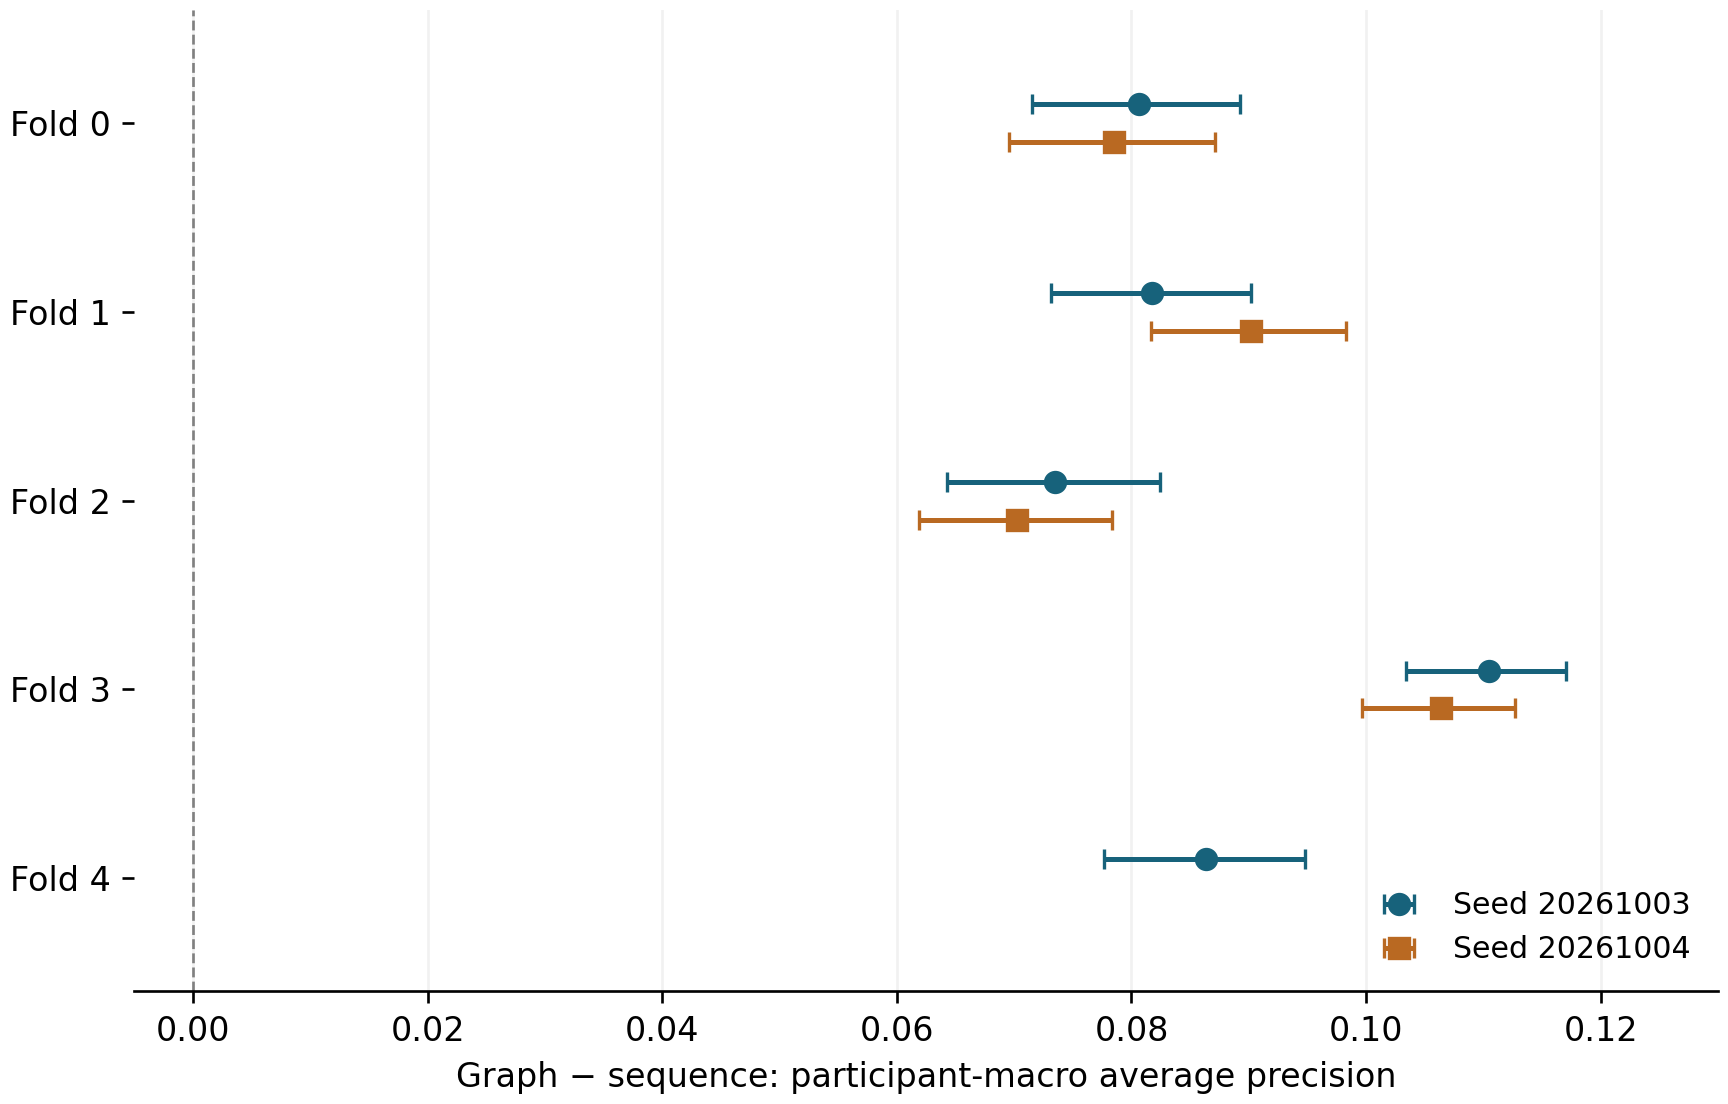
\includegraphics[width=.94\linewidth]{figures/ap_differences.png}\par\small
\textbf{Figure 1.} Graph-minus-sequence differences in participant-macro AP for all completed Apple MPS pairs at the evidence snapshot. Bars show 95\% participant-bootstrap intervals conditional on fitted predictions. Filled circles indicate seed 20261003; squares indicate seed 20261004. Seed 20261004 has no completed fold-4 pair in this snapshot. There is no pooled-effect marker because training sets overlap and seed coverage is incomplete.

\end{figure}
\subsection*{3.3. Second-seed and cross-hardware results}
At seed 20261004, completed pairs on folds 0--3 favored the graph on both AP and macro Brier (Table 3). This provides initial seed replication beyond a single fold. Coverage remained incomplete, and two seeds do not provide a reliable estimate of training-seed uncertainty. Repeated predictions for a participant under different seeds were not counted as additional independent participants.

\textbf{Table 3. Completed second-seed comparisons, seed 20261004.}

{\small
\setlength{\tabcolsep}{3pt}
\begin{longtable}{>{\raggedright\arraybackslash}p{\dimexpr 0.070\linewidth-2\tabcolsep\relax}>{\raggedright\arraybackslash}p{\dimexpr 0.120\linewidth-2\tabcolsep\relax}>{\raggedright\arraybackslash}p{\dimexpr 0.120\linewidth-2\tabcolsep\relax}>{\raggedright\arraybackslash}p{\dimexpr 0.345\linewidth-2\tabcolsep\relax}>{\raggedright\arraybackslash}p{\dimexpr 0.345\linewidth-2\tabcolsep\relax}}
\toprule
\textbf{Fold} & \textbf{Graph AP} & \textbf{Sequence AP} & \textbf{AP difference (95\% interval)} & \textbf{Macro-Brier difference (95\% interval)} \\ \midrule
\endhead
0 & 0.473152 & 0.394613 & +0.078540 (+0.069529, +0.087102) & -0.002178 (-0.002464, -0.001901) \\
1 & 0.459892 & 0.369684 & +0.090208 (+0.081627, +0.098271) & -0.002430 (-0.002807, -0.002070) \\
2 & 0.443559 & 0.373283 & +0.070275 (+0.061924, +0.078368) & -0.001721 (-0.001970, -0.001469) \\
3 & 0.468932 & 0.362545 & +0.106387 (+0.099619, +0.112682) & -0.002504 (-0.002872, -0.002147) \\
\bottomrule
\end{longtable}
}
All settings match the one-epoch Apple MPS comparison. Confidence intervals use 10,000 paired participant resamples and do not quantify uncertainty over seeds. The second-seed fold-4 result is pending in the manuscript evidence snapshot.

The earlier CUDA fold-0 comparison yielded graph AP 0.474481 versus sequence AP 0.389901, difference +0.084580 (95\% interval +0.078104 to +0.090816). Macro Brier was 0.021522 versus 0.024211, respectively. The MPS refit at the same seed and fold reproduced the direction, with AP difference +0.080620. Numerical outputs differed across hardware and execution conditions, so the CUDA and MPS results are presented separately. Their agreement supports execution robustness for this comparison, without expanding cohort diversity or demonstrating exact hardware reproducibility.

\subsection*{3.4. Modality-typed versus generic routing}
The one-fold CUDA routing pilot used the same graph topology and 36,883-parameter expert bank in both variants. Generic routing achieved macro AP 0.474481 and macro Brier 0.021522; modality-typed routing achieved AP 0.471859 and Brier 0.021619. The typed-minus-generic AP difference was -0.002622 (95\% interval -0.003386 to -0.001909), and the macro-Brier difference was +0.000097 (95\% interval +0.000076 to +0.000121). Typed AP was higher for 35 participants and lower for 95.

The tested routing constraint therefore did not improve performance. Because the labels were derived from information already present in the event tokens, this was a test of modality-specific parameter routing rather than additional clinical knowledge. The result cannot establish whether richer clinical relations, relation reconstruction controls, or a different training budget would change performance. The typed pilot's raw bundle was documented remotely; its local summary was available, but local raw-prediction recovery was not confirmed in this manuscript snapshot.

\subsection*{3.5. Earlier CGM and event diagnostics}
The corrected two-feature CGM logistic benchmark achieved participant-macro AP 0.446938 across 650 AP-defined participants and pooled Brier 0.021590 across 44,028,064 development windows. The persistence/slope score achieved AP 0.209095 and pooled Brier 0.055132 under that earlier development-test aggregation. These establish historical references but are not training-budget-matched graph comparisons.

On the common fold-0 validation set, adding fourteen recorded-event summary features to logistic regression reduced AP from 0.457055 to 0.425768. A selected additive residual fitted on top of frozen CGM logits also reduced AP, to 0.444091, although pooled Brier improved from 0.022880 to 0.022503. These results show that ranking and probabilistic error can move in different directions and that adding event summaries alone did not establish an AP benefit.

In a separate two-epoch full-history comparison, a CGM-only GRU achieved AP 0.471865 and macro Brier 0.021357, compared with AP 0.460532 and Brier 0.021839 for a joint CGM/event sequence model. A same-architecture event-disabled variant achieved AP 0.469458; the event-enabled-minus-disabled AP difference was -0.008926 (95\% interval -0.010402 to -0.007357). The disabled branch also removed event-encoder gradients, limiting effective-capacity equivalence. The joint event model improved from AP 0.397077 at epoch 1 to 0.460532 at epoch 2, demonstrating sensitivity to training duration. These diagnostics were not used to claim a graph advantage over a converged CGM-only model, nor do they show that auxiliary events are generally uninformative.

\section*{4. Discussion}
The principal finding is a consistent development advantage for the tested temporal event graph over a parameter-matched late-fusion sequence implementation. Directional agreement across all five validation folds at one seed, four completed folds at another seed, and a separate CUDA execution strengthens the case for further controlled evaluation. The evidence is broader than a single favorable fold. It remains specific to the present cohort, endpoint, information policy, implementations, and one-epoch budget.

The positive graph-versus-sequence contrast and negative typed-routing result address different mechanisms. Linking events to observed CGM positions provides an explicit alignment before temporal encoding; this may make event context easier to use under the tested optimization schedule. The generic model also averages an expert bank, whereas the non-graph model summarizes its event stream separately. Either difference could contribute. The experiments do not isolate graph message passing from early fusion, deterministic position alignment, or optimization behavior. A non-graph comparator with reconstructed event-to-CGM alignment, event-order perturbations, and constrained relation or edge shuffling is needed to determine which structural choice accounts for the advantage.

The typed-routing pilot provides no evidence that modality-specific expert selection improves prediction. Both variants already receive modality and timing information. Thus, even a positive typed-routing result would support an inductive-bias claim, not discovery of new clinical facts. Broad patient-centered knowledge graph, semantic integration, and graph-recurrent glucose forecasting ideas already appear in prior work [4--6]. Our contribution at this stage is the controlled retrospective comparison and its auditable information contract, rather than a claim of the first diabetes knowledge graph or a validated semantic explanation system.

The earlier event diagnostics make a simple “more modalities are better” interpretation implausible. Linear summaries and additive residuals did not improve AP, and the two-epoch sequence comparison favored CGM-only history. These findings do not contradict the present graph advantage over a particular event-sequence model: a representation can outperform another multimodal representation without establishing incremental value beyond an equally optimized CGM-only predictor. A matched graph-without-events control and a competitive CGM-only model trained under the same schedule remain necessary. Moreover, improvement between epochs in the historical models indicates that one epoch may compare rates of learning as much as attainable performance.

The data pipeline is central to interpreting these comparisons. Repeated uploads can overweight copied events, conflicting CGM values can affect targets, and incomplete futures can create outcome misclassification if treated as negative. Shared canonicalization, eligibility masks, and prediction identities reduce these risks. They do not establish complete event capture or validate all glucose extremes. The use of occurrence-time replay is especially consequential: manually entered carbohydrate events may only become usable later. Without measured arrival times, the present result is an optimistic retrospective benchmark. A delayed-availability sensitivity would be a simulation unless independently observed arrival metadata become available.

Clinical usefulness remains unmeasured. AP evaluates ranking under the retained outcome prevalence; Brier measures probabilistic error. Neither provides a threshold, false-alert rate, sustained-episode sensitivity, or achievable warning time. Before deployment-oriented interpretation, the protocol requires chronologically simulated alerts, validation-selected thresholds, refractory rules, and episode matching with documented observable follow-up. Calibration curves and any recalibration must also be evaluated without using final test outcomes to choose settings. No dosing recommendation or treatment effect follows from these risk predictions.

\subsection*{4.1. Limitations}
This study has several material limitations. First, all reported neural comparisons are exploratory development results. Architecture and representation decisions were informed by earlier development analyses, and the current comparisons are not untouched nested cross-validation. The separate final-performance group has not provided a reported model evaluation, and external validation has not been performed.

Second, neural fits used one epoch in the principal comparison, incomplete coverage of a second seed, and a fixed optimizer. We have not established convergence, equal optimization opportunity, or superiority over strong contemporary sequence architectures. Parameter matching cannot eliminate differences in computation, fusion position, chronological encoding, or effective model capacity. Source fingerprints are preserved, but the current manuscript preparation did not reproduce every prediction from its checkpoint.

Third, bootstrap intervals resample participants with fixed predictions. They do not capture model refitting, seed uncertainty, or model-selection effects. Fold training sets overlap, and second-seed comparisons reuse the same participants. Millions of overlapping windows do not substitute for independent participants or episodes.

Fourth, the population was selected for recorded modality presence and sufficiently observed CGM windows. We did not establish complete clinical event capture, characterize demographic subgroup performance, or verify generalization to other insulin delivery settings, devices, or healthcare populations. No demographic balance table or symptom ascertainment was available in the verified experiment summaries.

Fifth, immediate event availability was assumed, the primary numeric-range policy retains values without a device-specific validity cutoff, and subtype hashing may merge distinct source categories. The two-hour lookback and 64-event cap also bound the represented physiology. Reporting delay, range sensitivity, longer histories, and strict modality-complete subgroups remain unreported model sensitivities.

Finally, clinical relation semantics, explanation faithfulness, patient or clinician usability, alert burden, and prospective benefit have not been demonstrated. The deterministic event-to-CGM topology should not be interpreted causally. These limitations prevent presenting the current artifact as a clinically validated or explainable decision-support system.

\section*{5. Conclusions}
A temporal event-to-CGM graph outperformed a non-graph sequence predictor with the same recorded inputs and exact parameter count across five development folds at one seed and four completed folds at a second seed. Modality-specific routing did not improve over a generic edge operation in the separate pilot. The results support continued investigation of explicit event alignment and message aggregation, while leaving clinical semantic value, incremental benefit beyond an optimized CGM-only predictor, explanation fidelity, and final generalization unresolved.

\section*{Declarations}
\textbf{Ethics and consent:} This manuscript concerns secondary analysis of a public-use Loop release. The original prospective study reported institutional review board approval and electronic consent [2]. [AUTHOR TO INSERT: the local determination for this secondary analysis, including institution, review or exemption identifier, applicable data-use terms, and any required consent statement.] Original-study approval must not be presented as approval of this secondary analysis.

\textbf{Data availability:} The source release is associated with the Jaeb public dataset collection [3]. Access and reuse remain subject to the custodian's applicable terms. Participant-level caches, identifiers, checkpoints containing protected metadata, and prediction shards remain in protected local storage. [AUTHOR TO CONFIRM: the permitted public data-access statement and precise release citation.] Aggregate tables and an identifier-free evidence map accompany this draft.

\textbf{Code availability:} The project contains canonicalization, temporal eligibility, caching, training, pairing, and metric utilities, together with software tests. [AUTHOR TO INSERT: a public repository URL, archived version or DOI, environment specification, and code license after an appropriate release review.] The supplied manuscript build script reproduces the tables and figures from the existing aggregate audit files; it is not a replacement for the full model-training workflow.

\textbf{Funding:} [AUTHOR TO CONFIRM FUNDING SOURCES AND GRANT NUMBERS, OR AN ACCURATE NO-FUNDING STATEMENT.]

\textbf{Competing interests:} [EACH AUTHOR TO PROVIDE A DECLARATION.]

\textbf{Author contributions:} [AUTHOR TO COMPLETE CONTRIBUTOR ROLES AND APPROVE AUTHORSHIP ORDER.]

\textbf{Patient and public involvement:} [AUTHOR TO CONFIRM WHETHER PATIENTS OR THE PUBLIC CONTRIBUTED TO THIS SECONDARY ANALYSIS.]

\textbf{Acknowledgments and AI assistance:} [AUTHOR TO CONFIRM ACKNOWLEDGMENTS.] An AI assistant supported preparation of this working draft, reference checking, and extraction and formatting of existing aggregate results. The authors must verify all statements, approve the analysis and manuscript, and adapt this disclosure to the target journal's policy. No new model training was undertaken during preparation of this draft.

\section*{References}
[1] Battelino T, Danne T, Bergenstal RM, et al. Clinical Targets for Continuous Glucose Monitoring Data Interpretation: Recommendations From the International Consensus on Time in Range. Diabetes Care. 2019;42(8):1593--1603. \href{https://doi.org/10.2337/dci19-0028}{doi:10.2337/dci19-0028}.

[2] Lum JW, Bailey RJ, Barnes-Lomen V, et al. A Real-World Prospective Study of the Safety and Effectiveness of the Loop Open Source Automated Insulin Delivery System. Diabetes Technology \& Therapeutics. 2021;23(5):367--375. \href{https://doi.org/10.1089/dia.2020.0535}{doi:10.1089/dia.2020.0535}.

[3] Jaeb Center for Health Research. Public datasets: diabetes. Loop study public dataset, release dated 31 January 2023, as identified in the local release. \href{https://public.jaeb.org/datasets/diabetes}{Custodian dataset collection}. Accessed 20 October 2026. The custodian's collection page was checked; a standalone release DOI was not established.

[4] Daniel Onwuchekwa JI, Weber C, Maleshkova M. Enhancing Hypoglycemia Prediction in Type 1 Diabetes through Semantic Knowledge Integration and Machine Learning Optimization. ESWC 2024 conference-hosted manuscript. \href{https://2024.eswc-conferences.org/wp-content/uploads/2024/05/77770363.pdf}{Conference full text}. The PDF title is used rather than its shorter running header, “Semantic AI for Hypoglycemia Prediction in T1D.”

[5] Sarani Rad F, Hendawi R, Yang X, Li J. Personalized Diabetes Management with Digital Twins: A Patient-Centric Knowledge Graph Approach. Journal of Personalized Medicine. 2024;14(4):359. \href{https://doi.org/10.3390/jpm14040359}{doi:10.3390/jpm14040359}.

[6] Piao C, Zhu T, Baldeweg SE, et al. GARNN: An interpretable graph attentive recurrent neural network for predicting blood glucose levels via multivariate time series. Neural Networks. 2025;185:107229. \href{https://doi.org/10.1016/j.neunet.2025.107229}{doi:10.1016/j.neunet.2025.107229}.

[7] Rehman NU, Contreras I, Beneyto A, Vehi J. Explainable cluster-based learning for prediction of postprandial glycemic events and insulin dose optimization in type 1 diabetes. PLOS Digital Health. 2025;4(9):e0000996. \href{https://doi.org/10.1371/journal.pdig.0000996}{doi:10.1371/journal.pdig.0000996}.

[8] Gallardo-García C, Hernando ME, Subías D, Rigla M, García-Sáez G. Interpretable Multihorizon Glucose Forecasting for Assessing Nutritional Information Impact in Type 1 Diabetes Management: Model Development and Validation Study. JMIR AI. 2026;5:e105049. \href{https://doi.org/10.2196/105049}{doi:10.2196/105049}.

[9] Collins GS, Moons KGM, Dhiman P, et al. TRIPOD+AI statement: updated guidance for reporting clinical prediction models that use regression or machine learning methods. BMJ. 2024;385:e078378. \href{https://doi.org/10.1136/bmj-2023-078378}{doi:10.1136/bmj-2023-078378}.

\end{document}
